% ── 2 Desenvolvimento ───────────────────────────────────────────────────────
\chapter{DESENVOLVIMENTO}

% ═══════════════════════════════════════════════════════════════════════════════
\section[Objetivos]{OBJETIVOS}
% ═══════════════════════════════════════════════════════════════════════════════

O objetivo geral deste projeto é evoluir o sistema Leciona, desenvolvido inicialmente no Projeto Integrador II, para uma plataforma de gestão escolar operacional com deploy em nuvem, capaz de garantir a integridade da alocação de horários por meio de restrições a nível de banco de dados e testes automatizados, além de disponibilizar uma API RESTful para consumo descentralizado dos dados de horários, ausências e substituições.

Para alcançar esse objetivo geral, foram definidos os seguintes objetivos específicos:

\begin{enumerate}
    \item Refatorar a arquitetura do sistema em módulos independentes (\textit{core}, \textit{schedule}, \textit{attendance}, \textit{communication}), aplicando princípios SOLID de responsabilidade única e separação de interesses.
    \item Implementar restrições de integridade a nível de banco de dados (UniqueConstraint, ForeignKey, validações customizadas) para impedir choques de horários entre professores e entre turmas.
    \item Desenvolver um dashboard analítico com gráficos dinâmicos (Chart.js 4.x) para visualização de indicadores de ausências, substituições e distribuição de turmas por período.
    \item Conteinerizar a aplicação com Docker e Docker Compose, garantindo paridade entre os ambientes de desenvolvimento, teste e produção.
    \item Criar endpoints de API RESTful (JSON) para consumo assíncrono de dados de horários e faltas por interfaces externas.
    \item Implementar pipeline de Integração Contínua via GitHub Actions para execução automática de testes a cada \textit{push}.
    \item Desenvolver funcionalidade de exportação de relatórios em PDF (ReportLab), com cabeçalho institucional, tabela de dados e rodapé com data de emissão.
    \item Validar a solução junto à comunidade escolar da Escola Municipal Patrícia Viviani, coletando \textit{feedback} para iterações futuras.
\end{enumerate}


% ═══════════════════════════════════════════════════════════════════════════════
\section[Justificativa e delimitação do problema]{JUSTIFICATIVA E DELIMITAÇÃO DO PROBLEMA}
% ═══════════════════════════════════════════════════════════════════════════════

A pergunta norteadora desta pesquisa pode ser formulada da seguinte maneira: como garantir a alta disponibilidade, a integridade de dados e a facilidade de integração em um sistema de alocação de substituições emergenciais de professores em escolas públicas municipais?

A Escola Municipal Patrícia Viviani, localizada no bairro Topolândia, em São Sebastião (SP), atende alunos do Ensino Fundamental em múltiplas turmas distribuídas nos turnos matutino, vespertino e integral. A equipe administrativa da escola, composta pela Vice-Diretora Marília Izabel e por funcionários de secretaria, é responsável por organizar diariamente a grade de aulas. Quando um professor comunica ausência (por atestado médico, licença, luto ou outro motivo), essa equipe precisa, no mesmo dia, verificar os horários descobertos, localizar substitutos disponíveis e redistribuir a grade. Todo esse processo é feito manualmente, com anotações em cadernos e planilhas impressas, e a comunicação das substituições ocorre por meio de mensagens informais em aplicativos de celular, sem garantia de que todos os envolvidos recebam a informação a tempo.

As consequências desse fluxo manual são concretas. Turmas ficam sem professor quando a substituição não é alocada com rapidez suficiente. Choques de horários acontecem porque não há mecanismo que impeça a alocação de um mesmo substituto em duas turmas simultaneamente. A secretaria dedica parte significativa do expediente a tarefas que poderiam ser automatizadas, desviando esforço de outras demandas administrativas. Além disso, a ausência de dados consolidados impede que a coordenação identifique padrões recorrentes de falta (por exemplo, concentrações em determinados dias da semana ou períodos do ano) que poderiam subsidiar ações preventivas.

Do ponto de vista acadêmico, o projeto oferece ao grupo a oportunidade de aplicar, em um cenário real, conceitos estudados ao longo do curso de Tecnologia da Informação: modelagem de banco de dados relacional com restrições de integridade (ELMASRI; NAVATHE, 2011), desenvolvimento web seguindo o padrão arquitetural MTV do Django (DJANGO SOFTWARE FOUNDATION, 2025), conteinerização de aplicações com Docker (DOCKER INC., 2024), construção de API RESTful (FIELDING, 2000) e práticas de integração contínua (HUMBLE; FARLEY, 2010). A intersecção entre engenharia de software e gestão escolar permite que o grupo vivencie o ciclo completo de desenvolvimento, desde a elicitação de requisitos junto ao usuário final até o deploy e a coleta de \textit{feedback}.

A contribuição prática do projeto se materializa em um sistema gratuito e acessível via navegador, que centraliza o registro de ausências, automatiza a verificação de conflitos de horários, gera relatórios em PDF e apresenta indicadores visuais em um painel analítico. Por ser conteinerizado, o sistema pode ser implantado em qualquer provedor de nuvem sem ajustes na configuração. A escola parceira passa a contar com uma ferramenta que reduz o retrabalho da secretaria e fornece dados para a gestão.

O projeto dá continuidade ao trabalho realizado no Projeto Integrador II, quando o grupo construiu o protótipo inicial do Leciona. Naquela etapa, a Vice-Diretora Marília Izabel validou a proposta e indicou melhorias prioritárias, como a necessidade de acesso remoto (o protótipo funcionava apenas localmente), a visualização consolidada de faltas por período e a comunicação estruturada de substituições. Essas demandas orientaram o escopo do PI3, que concentra esforços na conteinerização, na API e no dashboard analítico.

Cabe registrar que o sistema lida com dados pessoais de professores (nome e telefone). A coleta dessas informações foi autorizada por meio de Termo de Consentimento Livre e Esclarecido (TCLE) aplicado junto aos participantes. O banco de dados PostgreSQL oferece mecanismos de controle de acesso e criptografia de conexão que contribuem para a proteção desses dados, em conformidade com os princípios da Lei Geral de Proteção de Dados Pessoais (LGPD).


% ═══════════════════════════════════════════════════════════════════════════════
\section[Fundamentação teórica]{FUNDAMENTAÇÃO TEÓRICA}
% ═══════════════════════════════════════════════════════════════════════════════

% ---------------------------------------------------------------------------
\subsection{Gestão escolar e tecnologia da informação}
% ---------------------------------------------------------------------------

A gestão escolar, segundo Lück (2009), não se restringe à administração de recursos financeiros e materiais. Ela envolve a articulação de processos pedagógicos, administrativos e comunitários, de modo que as decisões tomadas pela equipe gestora repercutam diretamente na qualidade do ensino oferecido aos alunos. A autora enfatiza que uma gestão eficaz depende da capacidade de integrar essas dimensões, o que exige instrumentos de organização que vão além do caderno de anotações e da planilha impressa.

Nas escolas públicas municipais brasileiras, as dificuldades administrativas são agravadas pela escassez de recursos humanos e tecnológicos. Coordenadores e secretários acumulam funções que incluem controle de frequência docente, organização de grades horárias, registro de matrículas e comunicação com pais e professores. Quando essas tarefas dependem exclusivamente de processos manuais, o risco de erros aumenta e o tempo disponível para atividades de planejamento pedagógico diminui. A falta de registros digitais centralizados impede, ainda, a construção de indicadores que poderiam orientar decisões da coordenação.

Moran (2015) argumenta que a incorporação de tecnologias digitais na educação precisa ir além da sala de aula e alcançar os processos de gestão institucional. O autor defende que sistemas informatizados aplicados à administração escolar podem acelerar rotinas operacionais, reduzir a incidência de falhas humanas e gerar dados que subsidiem a tomada de decisão. A digitalização dos processos de gestão, contudo, precisa considerar a realidade local da escola: infraestrutura de rede, familiaridade da equipe com ferramentas digitais e a necessidade de interfaces acessíveis que não imponham uma curva de aprendizado íngreme.

\begin{citacao}
A gestão escolar constitui uma dimensão e um enfoque de atuação em educação, que objetiva promover a organização, a mobilização e a articulação de todas as condições materiais e humanas necessárias para garantir o avanço dos processos socioeducacionais dos estabelecimentos de ensino, orientados para a promoção efetiva da aprendizagem dos alunos (LÜCK, 2009, p. 24).
\end{citacao}

Essa definição reforça que a gestão escolar não é um fim em si, mas um meio para viabilizar o processo educacional. Nesse enquadramento, um sistema como o Leciona atua como instrumento de apoio, automatizando tarefas repetitivas (registro de faltas, verificação de disponibilidade de substitutos, geração de relatórios) para que a equipe gestora possa concentrar seus esforços nas decisões pedagógicas.

% ---------------------------------------------------------------------------
\subsection{Desenvolvimento web com o framework Django}
% ---------------------------------------------------------------------------

O Django é um \textit{framework} web de alto nível, escrito em Python, que segue o padrão arquitetural MTV (Model-Template-View). Nesse padrão, o Model define a estrutura dos dados e as regras de validação, o Template é responsável pela camada de apresentação (HTML renderizado), e a View atua como intermediária, recebendo requisições HTTP, consultando os modelos e retornando respostas ao cliente. Embora a nomenclatura difira do padrão MVC (Model-View-Controller) amplamente documentado na literatura de engenharia de software, a correspondência funcional é direta: o Template do Django equivale à View do MVC, e a View do Django equivale ao Controller (DJANGO SOFTWARE FOUNDATION, 2025).

O ciclo de uma requisição no Django segue um fluxo bem definido. O servidor recebe a requisição HTTP e a encaminha ao sistema de roteamento (URLconf), que mapeia a URL para uma View específica. A View processa a lógica de negócio, interage com o banco de dados por meio do ORM (Object-Relational Mapping) e passa os dados para o Template, que gera o HTML de resposta. Esse ORM permite que o desenvolvedor manipule registros do banco de dados usando objetos Python, sem a necessidade de escrever SQL manualmente na maioria das operações. Consultas mais elaboradas, como agregações com \texttt{ExtractMonth} e \texttt{ExtractIsoWeekDay} (utilizadas no dashboard do Leciona), também são suportadas pela API de consultas do Django.

A modularização do sistema em aplicações Django independentes segue os princípios SOLID descritos por Martin (2009). O Princípio da Responsabilidade Única (SRP) orienta que cada módulo deve ter um, e apenas um, motivo para mudar. No Leciona, o módulo \textit{core} concentra as entidades fundamentais (Teacher, Subject, ClassGroup, SchoolSegment, SchoolPeriod, Justification), o módulo \textit{schedule} cuida exclusivamente da alocação de horários, o módulo \textit{attendance} gerencia ausências e substituições, e o módulo \textit{communication} trata do envio de comunicados. Essa separação permite que alterações em um módulo (por exemplo, a adição de um novo tipo de comunicado) não afetem o funcionamento dos demais.

A Django Software Foundation mantém documentação oficial extensa e atualizada, cobrindo desde a instalação até funcionalidades avançadas como \textit{middleware}, sinais, \textit{managers} customizados e o sistema de administração automática. Essa documentação, associada a uma comunidade ativa e a um ciclo de lançamento previsível, torna o Django uma escolha adequada para projetos acadêmicos que precisam de uma base madura e bem documentada (DJANGO SOFTWARE FOUNDATION, 2025).

% ---------------------------------------------------------------------------
\subsection{Banco de dados relacional e integridade referencial}
% ---------------------------------------------------------------------------

O modelo relacional, formalizado por Codd (1970) e amplamente detalhado por Elmasri e Navathe (2011), organiza os dados em tabelas (relações) compostas por linhas (tuplas) e colunas (atributos). As relações entre tabelas são estabelecidas por meio de chaves primárias e chaves estrangeiras, e a normalização do esquema reduz a redundância dos dados e as anomalias de atualização. A adoção de um SGBD relacional confere ao sistema um conjunto de garantias (as propriedades ACID: atomicidade, consistência, isolamento e durabilidade) que são fundamentais para aplicações que manipulam dados sensíveis, como registros de frequência docente.

O PostgreSQL, utilizado no Leciona, é um SGBD relacional de código aberto reconhecido pela robustez, pela conformidade com o padrão SQL e pelo suporte a funcionalidades avançadas como tipos de dados customizados, indexação parcial e extensões. Sua escolha neste projeto se justifica tanto pela maturidade do software quanto pela integração nativa com o ORM do Django, que gera automaticamente as migrações de esquema a partir dos modelos Python.

Um dos mecanismos centrais para garantir a integridade dos dados no Leciona é o uso de \textit{constraints} (restrições) definidas diretamente no banco. O modelo Schedule, por exemplo, possui duas restrições de unicidade (\texttt{UniqueConstraint}): a primeira impede que um professor seja alocado em duas turmas diferentes no mesmo dia e horário; a segunda impede que uma turma receba duas aulas simultâneas. Essas restrições são aplicadas pelo PostgreSQL no momento da inserção ou atualização dos dados, independentemente da camada de aplicação. Isso significa que, mesmo que uma validação na View ou no formulário falhe por algum motivo, o banco de dados impede a criação de registros inconsistentes (ELMASRI; NAVATHE, 2011).

Além das restrições de unicidade, o Leciona utiliza chaves estrangeiras (\texttt{ForeignKey}) para garantir a integridade referencial entre as tabelas. Uma ausência (\texttt{TeacherAbsence}) sempre referencia um professor e uma justificativa existentes; um horário (\texttt{Schedule}) sempre referencia uma turma, um professor e uma disciplina válidos. A indexação dos campos de data (\texttt{db\_index=True} em \texttt{start\_date} e \texttt{end\_date}) acelera as consultas de filtragem por período, que são frequentes nas operações de geração de relatórios e de alimentação dos gráficos do dashboard.

% ---------------------------------------------------------------------------
\subsection{API RESTful e arquitetura orientada a serviços}
% ---------------------------------------------------------------------------

O estilo arquitetural REST (Representational State Transfer), proposto por Fielding (2000) em sua tese de doutorado, define um conjunto de restrições para a construção de sistemas distribuídos na Web. Entre os princípios fundamentais estão a interface uniforme (uso padronizado dos métodos HTTP), a comunicação \textit{stateless} (cada requisição contém todas as informações necessárias para ser processada), a separação entre cliente e servidor, e a possibilidade de cache das respostas.

A adoção de uma API RESTful traz vantagens concretas para o Leciona. Ao expor os dados em formato JSON por meio de endpoints bem definidos, o sistema desacopla a camada de apresentação da lógica de negócio. O endpoint \texttt{/chartJSON/}, por exemplo, retorna os dados de ausências e substituições dos últimos seis meses em formato JSON, que são consumidos de forma assíncrona pelo Chart.js no navegador do usuário. Essa separação permite que, futuramente, aplicações móveis ou painéis externos consumam os mesmos dados sem alterações no \textit{backend}.

A interoperabilidade proporcionada pela API facilita a integração com outros sistemas eventualmente utilizados pela secretaria de educação do município. Pressman e Maxim (2016) destacam que a construção de interfaces bem definidas entre componentes de software é um dos pilares da engenharia de software moderna, pois reduz o acoplamento entre módulos e permite a evolução independente de cada parte do sistema. No contexto do Leciona, a API representa o primeiro passo para transformar o sistema de um painel web monolítico em uma plataforma orientada a serviços.

% ---------------------------------------------------------------------------
\subsection{Computação em nuvem e conteinerização}
% ---------------------------------------------------------------------------

O National Institute of Standards and Technology (NIST) define computação em nuvem como um modelo que permite o acesso ubíquo, conveniente e sob demanda a um conjunto compartilhado de recursos computacionais configuráveis (redes, servidores, armazenamento, aplicações e serviços) que podem ser provisionados e liberados rapidamente, com esforço mínimo de gerenciamento ou interação com o provedor de serviços (MELL; GRANCE, 2011). Essa definição abrange os modelos de serviço IaaS, PaaS e SaaS, e o Leciona se posiciona como uma aplicação que pode ser implantada em qualquer um desses modelos, graças à conteinerização.

O Docker é uma plataforma de conteinerização que empacota a aplicação e todas as suas dependências (sistema operacional base, bibliotecas, \textit{runtime} Python, pacotes) em uma imagem portátil. O Dockerfile do Leciona utiliza a imagem base \texttt{python:3.10-slim}, instala as dependências de sistema necessárias para a compilação do \texttt{psycopg2} (adaptador PostgreSQL para Python) e configura o Gunicorn como servidor WSGI com três \textit{workers} na porta 8080. Essa imagem pode ser executada em qualquer máquina que tenha o Docker instalado, eliminando o problema clássico de divergência entre ambientes de desenvolvimento e produção (DOCKER INC., 2024).

O Docker Compose, por sua vez, permite a definição de aplicações compostas por múltiplos contêineres em um único arquivo YAML (\texttt{docker-compose.yml}). No Leciona, o Compose orquestra dois serviços: \texttt{db} (PostgreSQL 15 Alpine, exposto na porta 5433) e \texttt{web} (aplicação Django, exposta na porta 8080). O volume \texttt{postgres\_data} garante a persistência dos dados do banco entre reinicializações dos contêineres. Com o comando \texttt{docker-compose up -d --build}, todo o ambiente é construído e iniciado automaticamente, o que simplifica tanto o desenvolvimento local quanto a implantação em servidores remotos.

Humble e Farley (2010) argumentam que a paridade entre ambientes é um pré-requisito para entregas confiáveis de software. Quando o ambiente de desenvolvimento difere do ambiente de produção em versões de bibliotecas, configurações de sistema operacional ou versões do banco de dados, erros que não se manifestam localmente podem surgir em produção. A conteinerização com Docker resolve esse problema ao garantir que o mesmo artefato (a imagem) é executado em todos os estágios do pipeline.

% ---------------------------------------------------------------------------
\subsection{Integração contínua e testes automatizados}
% ---------------------------------------------------------------------------

A Integração Contínua (CI), conforme definida por Humble e Farley (2010), é a prática de integrar o código de todos os desenvolvedores em um repositório compartilhado diversas vezes ao dia, executando uma \textit{build} automatizada (que inclui compilação, testes e verificações estáticas) a cada integração. O objetivo é detectar erros o mais cedo possível no ciclo de desenvolvimento, reduzindo o custo de correção e aumentando a confiança da equipe na base de código.

O GitHub Actions é a plataforma de CI/CD integrada ao GitHub que permite definir \textit{workflows} em arquivos YAML no diretório \texttt{.github/workflows/}. Cada \textit{workflow} é composto por \textit{jobs} que executam uma sequência de \textit{steps} em máquinas virtuais provisionadas sob demanda. Para o Leciona, o \textit{workflow} de CI é acionado a cada \textit{push} e a cada abertura de \textit{pull request}, executando a suíte de testes do Django em um ambiente com PostgreSQL configurado como serviço.

Os testes automatizados são a base da CI. Sommerville (2011) classifica os testes em unitários (que verificam o comportamento de componentes isolados), de integração (que verificam a interação entre componentes) e de sistema (que verificam o comportamento do sistema como um todo). No Leciona, os testes unitários validam regras de negócio críticas: a impossibilidade de um professor substituir a si mesmo (\texttt{TeacherSubstitution.clean()}), a obrigatoriedade de que a data de início preceda a data de término (\texttt{TeacherAbsence.clean()}), e a verificação de que o professor está habilitado a lecionar a disciplina atribuída (\texttt{Schedule.clean()}). As restrições de unicidade no banco de dados complementam esses testes, formando uma rede de proteção em duas camadas (aplicação e banco).

\begin{citacao}
Testing can only show the presence of errors, not their absence. Nevertheless, the value of software testing lies precisely in the systematic detection of faults that would otherwise reach production and affect users (SOMMERVILLE, 2011, p. 208).
\end{citacao}

Essa observação, que remonta ao trabalho de Dijkstra (1972), reforça a importância de combinar testes automatizados com outras estratégias de verificação, como revisão de código e \textit{constraints} de banco de dados, para maximizar a cobertura de detecção de erros.

% ---------------------------------------------------------------------------
\subsection{Acessibilidade web}
% ---------------------------------------------------------------------------

As Diretrizes de Acessibilidade para Conteúdo Web (WCAG) 2.1, publicadas pelo World Wide Web Consortium, estabelecem critérios técnicos para que conteúdos e interfaces web sejam acessíveis a pessoas com diferentes tipos de deficiência (W3C, 2018). As diretrizes estão organizadas em quatro princípios (perceptível, operável, compreensível e robusto) e três níveis de conformidade (A, AA e AAA). O nível AA é considerado referência para a maioria das aplicações web governamentais e educacionais.

O Leciona utiliza o Jazzmin como tema para o painel administrativo do Django. O Jazzmin é construído sobre o AdminLTE 3, que por sua vez é baseado no Bootstrap 4. Essa cadeia de dependências confere ao sistema uma interface responsiva, que se adapta a diferentes tamanhos de tela (desktops, tablets e smartphones), além de oferecer componentes com atributos ARIA (\textit{Accessible Rich Internet Applications}) que facilitam a interação por meio de leitores de tela. Os formulários do painel administrativo utilizam \textit{labels} associados a campos de entrada, contrastes de cor adequados e navegação por teclado.

A escolha de um tema baseado em Bootstrap também contribui para a consistência visual da interface. Elementos como botões, tabelas, cards e menus seguem um padrão visual uniforme, reduzindo a carga cognitiva do usuário. Para a equipe administrativa da escola, que pode não ter familiaridade com sistemas complexos, essa consistência facilita o aprendizado e a adoção da ferramenta. Moran (2015) destaca que a tecnologia aplicada à educação só cumpre seu papel quando é efetivamente utilizada pelos atores envolvidos, o que depende, em grande medida, da usabilidade e da acessibilidade da interface oferecida.


% ═══════════════════════════════════════════════════════════════════════════════
\section[Metodologia]{METODOLOGIA}
% ═══════════════════════════════════════════════════════════════════════════════

A metodologia adotada segue o Design Thinking proposto pela UNIVESP como framework para os Projetos Integradores, estruturado em três etapas: ouvir, criar e implementar. A seguir, descrevem-se as estratégias empregadas em cada etapa, os instrumentos de coleta de dados e as decisões técnicas tomadas durante o desenvolvimento.

\subsection{Ouvir e interpretar o contexto}

O projeto foi realizado em parceria com a Escola Municipal Patrícia Viviani, localizada no bairro Topolândia, em São Sebastião (SP). A escola atende turmas do Ensino Fundamental distribuídas nos turnos matutino, vespertino e integral, totalizando um corpo docente que ultrapassa trinta professores. A principal interlocutora do grupo na escola foi a Vice-Diretora Marília Izabel, que participou de todas as etapas de validação.

A coleta de informações ocorreu por meio de reuniões presenciais e remotas com a equipe administrativa da escola. Na primeira reunião, o grupo apresentou o protótipo desenvolvido no PI2 e solicitou que a Vice-Diretora avaliasse as funcionalidades existentes e indicasse lacunas. Antes da coleta formal de dados, foi aplicado o Termo de Consentimento Livre e Esclarecido (TCLE) a todos os participantes, garantindo o uso ético das informações fornecidas.

Os problemas levantados durante essa fase foram: (a) o registro manual de ausências de professores, que dependia de cadernos e planilhas sem padronização; (b) choques de horários causados pela alocação manual de substitutos, sem verificação de disponibilidade; (c) comunicação descentralizada, em que avisos de substituição eram transmitidos por mensagens informais, sem garantia de recebimento por todos os envolvidos; (d) ausência de dados consolidados para identificar padrões de falta por período, dia da semana ou justificativa. A Vice-Diretora também apontou que o protótipo do PI2, por funcionar apenas localmente, não era utilizável no cotidiano da escola.

A partir dessas informações, o grupo definiu as prioridades do PI3: conteinerizar a aplicação para permitir acesso remoto, implementar restrições de integridade no banco de dados para eliminar choques de horários, construir um dashboard com indicadores visuais e estruturar a comunicação de substituições por meio de um módulo dedicado.

\subsection{Criar e prototipar}

Com os requisitos refinados, o grupo tomou a decisão de refatorar a base de código existente, em vez de iniciar um novo projeto. Essa escolha se baseou em dois fatores: o aproveitamento das entidades e regras de negócio já modeladas no PI2, e a possibilidade de demonstrar a evolução de um sistema ao longo de seu ciclo de vida, conforme preconizado por Sommerville (2011).

A primeira decisão técnica foi a reorganização do código em quatro módulos Django com responsabilidades bem definidas. O módulo \textit{core} concentra as entidades fundamentais (Teacher, Subject, ClassGroup, SchoolSegment, SchoolPeriod, Justification). O módulo \textit{schedule} trata exclusivamente da alocação de horários, com o modelo Schedule e suas restrições de unicidade. O módulo \textit{attendance} gerencia o registro de ausências (TeacherAbsence) e substituições (TeacherSubstitution), incluindo validações que impedem a auto-substituição e verificam a consistência de datas. O módulo \textit{communication} cuida do envio de comunicados tipificados (comunicação, evento, observação, pedagógico), com possibilidade de vinculação a turmas e professores específicos.

A modelagem do banco de dados foi revisada para incorporar restrições de integridade diretamente no PostgreSQL. Além das chaves estrangeiras e das validações no método \texttt{clean()} dos modelos Django, foram adicionadas duas \texttt{UniqueConstraint} ao modelo Schedule, que impedem, respectivamente, a duplicação de um professor em duas turmas no mesmo horário e a duplicação de aulas em uma mesma turma no mesmo horário. Essas restrições atuam como camada de proteção adicional, independente da aplicação.

Para o dashboard, o grupo prototipou três gráficos utilizando Chart.js 4.x: um gráfico de linhas comparando ausências e substituições nos últimos seis meses, um gráfico de barras mostrando a distribuição de ausências por dia da semana, e um gráfico \textit{doughnut} com a distribuição de turmas por período. Os dados são obtidos por meio de consultas agregadas no banco (usando \texttt{ExtractMonth} e \texttt{ExtractIsoWeekDay} do ORM do Django) e entregues ao \textit{frontend} via JSON.

A conteinerização foi definida com Docker Compose, orquestrando dois serviços: o banco de dados PostgreSQL 15 Alpine e a aplicação Django servida pelo Gunicorn. A imagem Docker utiliza a base \texttt{python:3.10-slim} e instala apenas as dependências necessárias para compilação do \texttt{psycopg2} e da biblioteca Pillow, resultando em uma imagem leve e reprodutível.

Para facilitar o teste da interface e do dashboard, o grupo criou um comando de \textit{seed} (\texttt{python manage.py seed\_db}) que utiliza a biblioteca Faker com locale \texttt{pt\_BR} para gerar dados realistas: 40 professores com nomes e telefones brasileiros, 20 turmas distribuídas em quatro segmentos e quatro períodos, 11 disciplinas, 6 justificativas de ausência, horários de aula com tratamento de conflitos, 50 ausências distribuídas nos últimos seis meses (com 70\% de chance de substituição associada) e 20 comunicados.

\subsection{Implementar e testar}

A implementação seguiu a ordem definida na prototipação. A refatoração em módulos foi realizada primeiro, seguida pela adição das restrições de banco de dados, pela construção do dashboard, pela conteinerização e pela exportação de relatórios em PDF.

O deploy em Docker foi validado localmente com o comando \texttt{docker-compose up -d --build}, que constrói a imagem da aplicação, inicia o banco de dados PostgreSQL e expõe o sistema na porta 8080. O volume persistente \texttt{postgres\_data} garante que os dados do banco sobrevivam a reinicializações dos contêineres. O seed de dados foi executado dentro do contêiner web para popular o banco com dados de teste.

Os testes unitários foram direcionados às regras de negócio mais críticas: a validação de que um professor não pode substituir a si mesmo, a validação de que datas de início devem preceder datas de término, a verificação de que um professor só pode lecionar disciplinas para as quais está habilitado, e a aplicação das restrições de unicidade que impedem choques de horários. Esses testes são executados pelo \textit{test runner} do Django com banco de dados de teste em memória.

A apresentação do sistema à escola parceira foi planejada para a Quinzena 4 do calendário do PI3. O objetivo é coletar \textit{feedback} qualitativo da Vice-Diretora e da secretaria sobre a usabilidade do painel administrativo, a clareza dos gráficos do dashboard e a utilidade da funcionalidade de exportação em PDF. As sugestões recebidas serão priorizadas e incorporadas nas iterações seguintes, conforme a capacidade do grupo no período restante do semestre.


% ═══════════════════════════════════════════════════════════════════════════════
\section[Resultados preliminares: solução inicial]{RESULTADOS PRELIMINARES: SOLUÇÃO INICIAL}
% ═══════════════════════════════════════════════════════════════════════════════

Os resultados preliminares do projeto são apresentados a seguir, organizados conforme as três etapas da metodologia Design Thinking: ouvir, criar e implementar.

\subsection{Resultados da etapa de ouvir}

O contato com a Escola Municipal Patrícia Viviani permitiu identificar com precisão os problemas enfrentados pela equipe administrativa na gestão de ausências e substituições de professores. A Vice-Diretora Marília Izabel recebeu o protótipo do PI2 de forma positiva, destacando que a escola não possuía qualquer sistema digital voltado a esse tipo de controle. Ao mesmo tempo, indicou que a adoção efetiva dependeria de o sistema estar disponível em nuvem (acessível de qualquer computador da escola) e de oferecer garantias contra erros de alocação.

A Tabela \ref{tab:problemas} sintetiza os problemas identificados durante as reuniões com a escola.

\begin{table}[H]
\centering
\caption{Problemas identificados na gestão de ausências da escola parceira}
\label{tab:problemas}
\begin{tabular}{p{4cm}p{9cm}}
\toprule
\textbf{Problema} & \textbf{Descrição} \\
\midrule
Registro manual de ausências & Faltas de professores anotadas em cadernos ou planilhas, sem centralização digital \\
Choques de horários & Substituições alocadas manualmente, gerando sobreposição de professores em turmas diferentes no mesmo horário \\
Comunicação descentralizada & Avisos de substituição transmitidos por mensagens informais, sem garantia de que todos os envolvidos foram notificados \\
Ausência de histórico analítico & Sem dados consolidados para identificar padrões de ausência por período, dia da semana ou justificativa \\
\bottomrule
\end{tabular}
\end{table}

Esses problemas confirmaram a pertinência da proposta e orientaram as prioridades de desenvolvimento para o PI3. A demanda por confiabilidade (evitar choques) foi traduzida em restrições de banco de dados; a demanda por acesso remoto foi traduzida em conteinerização e deploy em nuvem; a demanda por histórico analítico foi traduzida no dashboard com gráficos.

\subsection{Resultados da etapa de criar}

A refatoração do código resultou em uma arquitetura modular composta por quatro aplicações Django independentes, cada uma com seus modelos, views, templates e arquivos de administração. A seguir, uma breve descrição de cada módulo:

\begin{itemize}
    \item \textbf{core:} contém os modelos fundamentais do sistema. O modelo Teacher armazena nome, telefone (validado por expressão regular) e uma relação \textit{many-to-many} com Subject, além de um campo booleano \texttt{is\_substitute} que identifica professores substitutos. Os modelos ClassGroup, SchoolSegment e SchoolPeriod representam, respectivamente, turmas, segmentos escolares e períodos (manhã, tarde, noite, integral). O modelo Justification armazena os tipos de justificativa para ausências (médica, pessoal, maternidade, trânsito, luto, jurídica).
    \item \textbf{schedule:} contém o modelo Schedule, que relaciona turma, professor, disciplina, dia da semana e horário (início e fim). Duas \texttt{UniqueConstraint} garantem, a nível de banco de dados, que um professor não pode estar em duas turmas no mesmo horário e que uma turma não pode ter duas aulas simultâneas. O método \texttt{clean()} valida adicionalmente que o professor está habilitado a lecionar a disciplina atribuída.
    \item \textbf{attendance:} contém os modelos TeacherAbsence e TeacherSubstitution. O primeiro registra ausências com datas indexadas (\texttt{db\_index=True}) e referência a professor e justificativa. O segundo registra substituições, com referências ao professor ausente e ao substituto. O método \texttt{clean()} de TeacherSubstitution impede que um professor substitua a si mesmo e valida a consistência das datas.
    \item \textbf{communication:} contém o modelo Message, que permite o registro de comunicados tipificados (comunicação, evento, observação, pedagógico), com data, descrição, imagem opcional e vinculação a turmas e professores por meio de relações \textit{many-to-many}.
\end{itemize}

O modelo de dados resultante reflete as regras de negócio levantadas junto à escola. As chaves estrangeiras garantem a integridade referencial, as restrições de unicidade previnem conflitos de alocação, e as validações nos métodos \texttt{clean()} complementam essas restrições com verificações que o banco de dados relacional não consegue expressar sozinho (como a validação de habilitação do professor para a disciplina).

\begin{figure}[H]
\centering
\resizebox{\textwidth}{!}{% ── Diagrama Entidade-Relacionamento (TikZ vetorial) ────────────────────────
%
% Layout: 3 colunas com corredores de 2 cm entre elas.
%
%   Coluna 1 (x=0)       Corredor 1       Coluna 2 (x=5)       Corredor 2       Coluna 3 (x=10)
%   x: -1.5 a 1.5        x: 1.5 a 3.5     x: 3.5 a 6.5         x: 6.5 a 8.5     x: 8.5 a 11.5
%
% Regra: TODAS as setas entre colunas usam apenas segmentos horizontais
% e verticais, trafegando exclusivamente pelos corredores.
%
\definecolor{coreBlue}{HTML}{3B82F6}
\definecolor{schedGreen}{HTML}{22C55E}
\definecolor{attRed}{HTML}{EF4444}
\definecolor{commAmber}{HTML}{F59E0B}

\tikzset{
  erd head/.style={
    rectangle, fill=#1, text=white, font=\bfseries\scriptsize,
    minimum width=3cm, minimum height=0.45cm, inner sep=2pt, anchor=north,
  },
  erd fields/.style={
    rectangle, draw=#1, fill=#1!4, line width=0.6pt,
    minimum width=3cm, inner sep=3pt, anchor=north,
    font=\tiny, text width=2.7cm, align=left,
  },
  fkarrow/.style={-{Stealth[length=4pt, width=3pt]}, semithick, #1!60!black},
  m2marrow/.style={{Stealth[length=4pt, width=3pt]}-{Stealth[length=4pt, width=3pt]}, semithick, #1!60!black, dashed},
  modlabel/.style={font=\scriptsize\bfseries\itshape, text=#1!80!black},
}

\newcommand{\ent}[5]{% name, color, title, fields, (x,y)
  \node[erd head=#2] (#1H) at (#5) {#3};
  \node[erd fields=#2, below=-0.6pt of #1H] (#1B) {#4};
  \node[fit=(#1H)(#1B), inner sep=0pt] (#1) {};
}

\begin{tikzpicture}[remember picture]

% ════════════════════════════════════════════════════════════════════
% COLUNA 1 (x = 0): entidades de referência do core
% ════════════════════════════════════════════════════════════════════

\ent{SS}{coreBlue}{SchoolSegment}{%
  \underline{id} : BigAutoField (PK)\\
  name : CharField(200)%
}{0, 0}

\ent{CG}{coreBlue}{ClassGroup}{%
  \underline{id} : BigAutoField (PK)\\
  name : CharField(200)\\
  segment : FK $\to$ SchoolSegment\\
  period : FK $\to$ SchoolPeriod%
}{0, -1.6}

\ent{SP}{coreBlue}{SchoolPeriod}{%
  \underline{id} : BigAutoField (PK)\\
  name : CharField(200)%
}{0, -3.8}

\ent{SU}{coreBlue}{Subject}{%
  \underline{id} : BigAutoField (PK)\\
  name : CharField(200)%
}{0, -5.4}

\ent{J}{coreBlue}{Justification}{%
  \underline{id} : BigAutoField (PK)\\
  name : CharField(200)%
}{0, -7}

% ════════════════════════════════════════════════════════════════════
% COLUNA 2 (x = 5): Teacher, Schedule, Message
% ════════════════════════════════════════════════════════════════════

\ent{T}{coreBlue}{Teacher}{%
  \underline{id} : BigAutoField (PK)\\
  name : CharField(200)\\
  phone : CharField(17)\\
  is\_substitute : BooleanField\\
  subjects : M2M $\to$ Subject%
}{5, 0}

\ent{SC}{schedGreen}{Schedule}{%
  \underline{id} : BigAutoField (PK)\\
  day\_of\_week : CharField(20)\\
  class\_group : FK $\to$ ClassGroup\\
  teacher : FK $\to$ Teacher\\
  subject : FK $\to$ Subject\\
  start\_time : TimeField\\
  end\_time : TimeField\\[1pt]
  {\itshape UC: teacher + day + start}\\
  {\itshape UC: class + day + start}%
}{5, -3}

\ent{M}{commAmber}{Message}{%
  \underline{id} : BigAutoField (PK)\\
  message\_type : CharField(20)\\
  date : DateField\\
  description : TextField\\
  image : ImageField (opcional)\\
  class\_groups : M2M $\to$ ClassGroup\\
  teachers : M2M $\to$ Teacher%
}{5, -7}

% ════════════════════════════════════════════════════════════════════
% COLUNA 3 (x = 10): attendance
% ════════════════════════════════════════════════════════════════════

\ent{TA}{attRed}{TeacherAbsence}{%
  \underline{id} : BigAutoField (PK)\\
  start\_date : DateField (idx)\\
  end\_date : DateField (idx)\\
  teacher : FK $\to$ Teacher\\
  justification : FK $\to$ Justification%
}{10, 0}

\ent{TS}{attRed}{TeacherSubstitution}{%
  \underline{id} : BigAutoField (PK)\\
  start\_date : DateField (idx)\\
  end\_date : DateField (idx)\\
  absent\_teacher : FK $\to$ Teacher\\
  substitute\_teacher : FK $\to$ Teacher%
}{10, -2.8}

% ════════════════════════════════════════════════════════════════════
% SETAS — apenas segmentos H e V, roteando pelos corredores
%
% Corredor 1 (entre col 1 e col 2): canais em x = 2.0, 2.4, 2.8, 3.2
% Corredor 2 (entre col 2 e col 3): canais em x = 7.0, 7.5, 8.0
% Corredor externo direito: x = 12
% ════════════════════════════════════════════════════════════════════

% ── Dentro da coluna 1 (vertical curta) ────────────────────────────

% 1. ClassGroup → SchoolSegment
\draw[fkarrow=coreBlue] (CGH.north) -- (SSB.south);

% 2. ClassGroup → SchoolPeriod
\draw[fkarrow=coreBlue] (CGB.south) -- (SPH.north);

% ── Dentro da coluna 2 (vertical curta) ────────────────────────────

% 3. Schedule → Teacher
\draw[fkarrow=schedGreen] (SCH.north) -- (TB.south);

% ── Pelo corredor 1: col 2 → col 1 ────────────────────────────────

% 4. Teacher ↔ Subject (M2M) — canal x = 2.5
\draw[m2marrow=coreBlue]
  ([yshift=2pt]T.west) -- (2.5, -0.7)
  -- (2.5, -5.7)
  -- ([yshift=2pt]SU.east);

% 5. Schedule → ClassGroup — canal x = 2.0
\draw[fkarrow=schedGreen]
  ([yshift=6pt]SC.west) -- (2.0, -3.8)
  -- (2.0, -2.4)
  -- ([yshift=-2pt]CG.east);

% 6. Schedule → Subject — canal x = 2.8
\draw[fkarrow=schedGreen]
  ([yshift=-6pt]SC.west) -- (2.8, -4.8)
  -- (2.8, -5.9)
  -- ([yshift=-2pt]SU.east);

% 7. Message ↔ ClassGroup (M2M) — canal x = 3.2
\draw[m2marrow=commAmber]
  ([yshift=6pt]M.west) -- (3.2, -7.2)
  -- (3.2, -2.8)
  -- ([yshift=-6pt]CG.east);

% ── Pelo corredor 2: col 3 → col 2 ────────────────────────────────

% 8. TeacherAbsence → Teacher — horizontal direta y = -0.8
\draw[fkarrow=attRed]
  (TA.west) -- (T.east);

% 9. TeacherSubstitution → Teacher — canal x = 7.2
\draw[fkarrow=attRed]
  (TS.west) -- (7.2, -3.6)
  -- (7.2, -1.3)
  -- ([yshift=-6pt]T.east);

% ── Pelo corredor 2: col 3 → col 2 (M2M) ─────────────────────────

% 10. Message ↔ Teacher (M2M) — canal x = 7.8
\draw[m2marrow=commAmber]
  ([yshift=-2pt]M.east) -- (7.8, -8.2)
  -- (7.8, -1.0)
  -- ([yshift=-2pt]T.east);

% ── Rota longa: col 3 → col 1 (pelo corredor externo) ─────────────

% 11. TeacherAbsence → Justification — contorna por fora (x=12, y=-6.5)
\draw[fkarrow=attRed]
  ([yshift=-2pt]TA.east) -- (12, -0.9)
  -- (12, -6.5)
  -- (1.5, -6.5)
  -- (1.5, -7.3)
  -- ([yshift=2pt]J.east);

% ════════════════════════════════════════════════════════════════════
% LABELS DE MÓDULO
% ════════════════════════════════════════════════════════════════════

\node[modlabel=coreBlue]   at (0, 0.6) {core};
\node[modlabel=coreBlue]   at (5, 0.6) {core};
\node[modlabel=schedGreen] at (5, -2.5) {schedule};
\node[modlabel=commAmber]  at (5, -6.5) {communication};
\node[modlabel=attRed]     at (10, 0.6) {attendance};

% ════════════════════════════════════════════════════════════════════
% LEGENDA
% ════════════════════════════════════════════════════════════════════

\node[anchor=north west, font=\tiny, inner sep=2pt] at (8.5, -5.5) {%
  \begin{tabular}{@{}r@{\enspace}l@{}}
  \tikz[baseline=-0.5ex]\draw[fkarrow=black] (0,0) -- (0.5,0); & Chave estrangeira (FK) \\[2pt]
  \tikz[baseline=-0.5ex]\draw[m2marrow=black] (0,0) -- (0.5,0); & Relacionamento M2M \\[2pt]
  \textit{UC} & UniqueConstraint \\[2pt]
  \textit{idx} & Campo indexado (db\_index) \\
  \end{tabular}%
};

\end{tikzpicture}
}
\caption{Diagrama entidade-relacionamento do sistema Leciona, organizado por módulo}
\label{fig:diagrama-er}
\end{figure}

A Figura \ref{fig:diagrama-er} apresenta o diagrama entidade-relacionamento do sistema, organizado por módulo. As cores identificam a qual aplicação Django cada entidade pertence: azul para o módulo \textit{core}, verde para \textit{schedule}, vermelho para \textit{attendance} e laranja para \textit{communication}. As setas contínuas representam chaves estrangeiras e as setas tracejadas representam relacionamentos muitos-para-muitos.

\subsection{Resultados da etapa de implementar}

A implementação produziu um sistema funcional que cobre os requisitos definidos nas etapas anteriores. Os principais resultados são detalhados a seguir.

\textbf{Dashboard analítico.} A view \texttt{DashboardView}, acessível em \texttt{/statistics/}, apresenta três gráficos construídos com Chart.js 4.x e cards com contadores de professores, turmas e segmentos cadastrados. O primeiro gráfico é uma linha temporal que compara o número de ausências registradas com o número de substituições realizadas nos últimos seis meses. Os dados são obtidos por meio de consultas agregadas que utilizam \texttt{ExtractMonth} para agrupar os registros por mês, e são servidos como JSON pelo endpoint \texttt{/chartJSON/} (uma view baseada em \texttt{BaseLineChartView}). O segundo gráfico é um gráfico de barras que mostra a distribuição de ausências por dia da semana (segunda a sexta), utilizando \texttt{ExtractIsoWeekDay} para extrair o dia da data de início de cada ausência. O terceiro gráfico é um \textit{doughnut} que exibe a distribuição de turmas por período escolar (manhã, tarde, noite, integral), permitindo que a coordenação visualize rapidamente o equilíbrio da oferta entre turnos.

\begin{figure}[H]
\centering
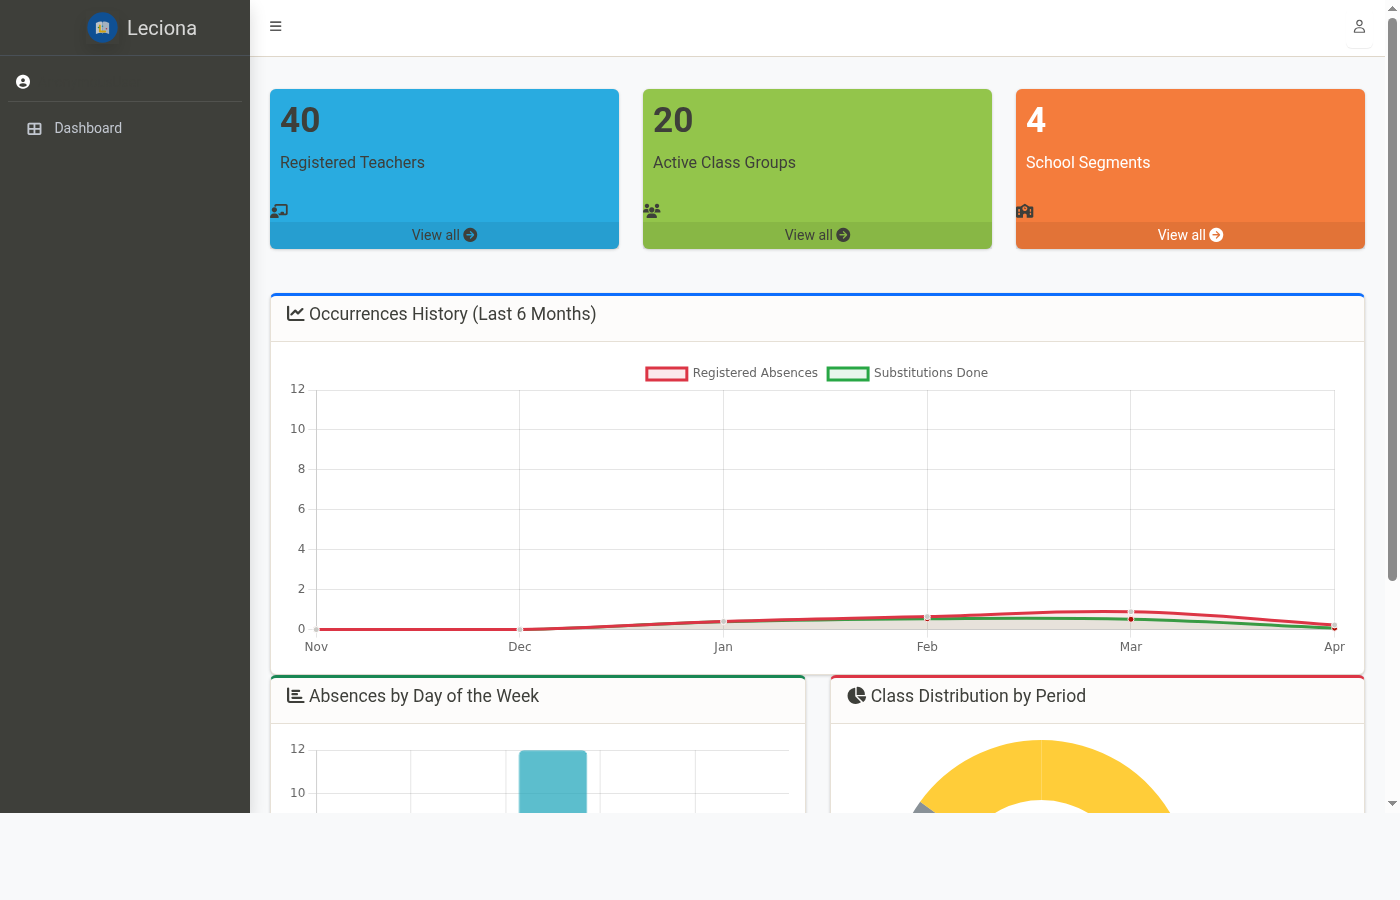
\includegraphics[width=0.9\textwidth]{images/dashboard.png}
\caption{Dashboard analítico do sistema Leciona com gráficos de ausências e substituições}
\label{fig:dashboard}
\end{figure}

\textbf{Painel administrativo.} O painel administrativo do Django, personalizado com o tema Jazzmin (baseado em AdminLTE 3 e Bootstrap 4), oferece interfaces de cadastro, edição e consulta para todas as entidades do sistema: professores, disciplinas, turmas, segmentos, períodos, justificativas, horários, ausências, substituições e comunicados. Cada entidade possui uma classe \texttt{ModelAdmin} registrada, com configuração de campos exibidos em lista (\texttt{list\_display}), filtros laterais (\texttt{list\_filter}) e ações customizadas. A navegação pelo painel é intuitiva, com menus laterais organizados por módulo e suporte a busca rápida.

\begin{figure}[H]
\centering
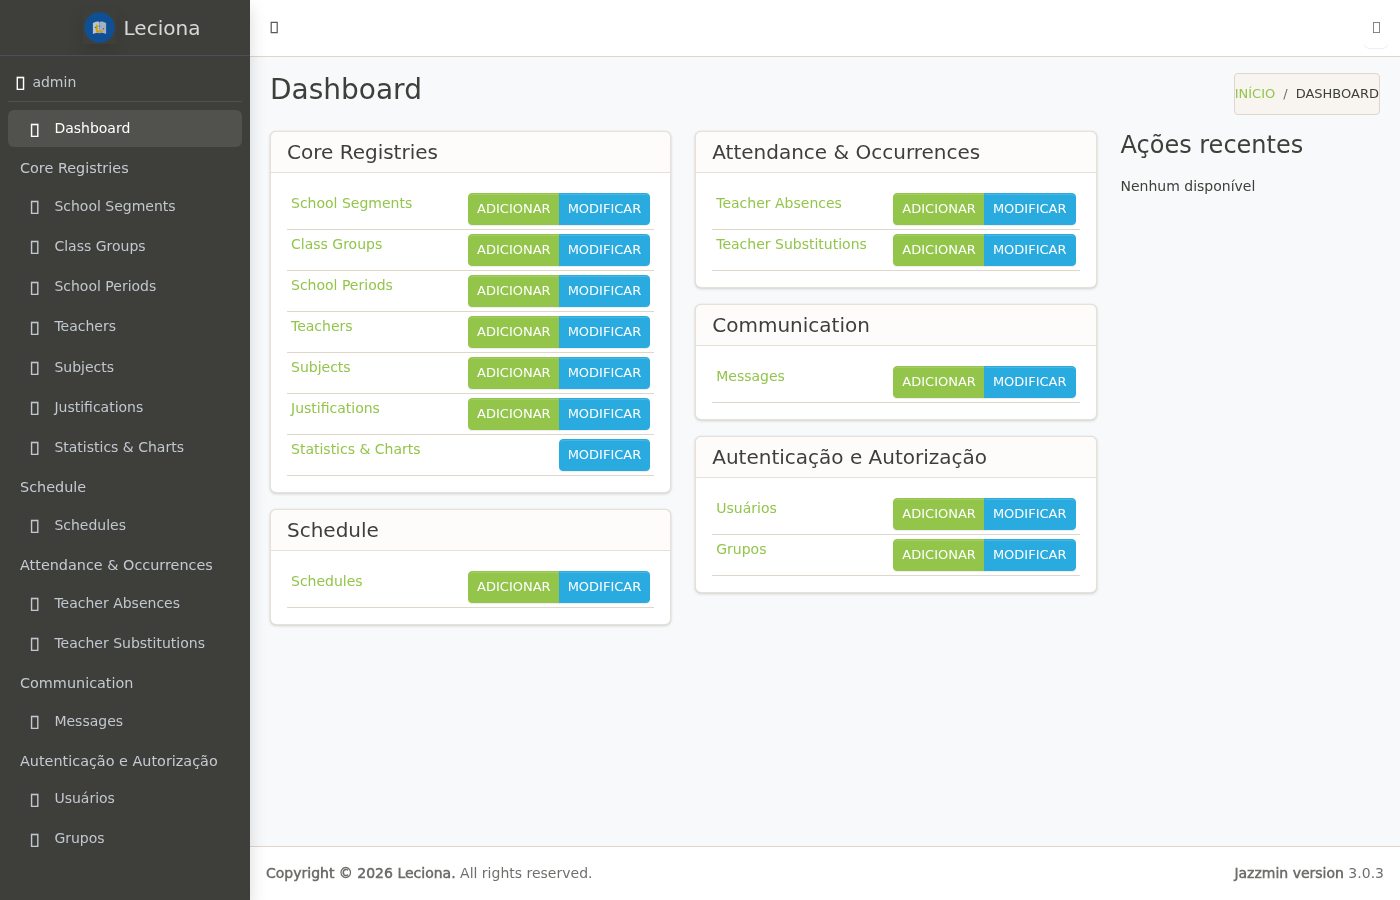
\includegraphics[width=0.9\textwidth]{images/admin-panel.png}
\caption{Painel administrativo do Leciona com tema Jazzmin}
\label{fig:admin}
\end{figure}

\textbf{Exportação de relatórios em PDF.} A funcionalidade de exportação em PDF foi implementada como uma ação customizada do Django Admin, disponível para todos os modelos registrados. A ação utiliza a biblioteca ReportLab para gerar documentos em formato A4 com cabeçalho institucional (logo do sistema e título), tabela com os dados selecionados, contagem total de registros e rodapé com data de emissão e nome do usuário que gerou o relatório. O administrador seleciona os registros desejados na lista, escolhe a ação ``Export to PDF'' e recebe o download do arquivo. Essa funcionalidade atende à demanda da secretaria por relatórios impressos de professores, turmas e ausências.

\begin{figure}[H]
\centering
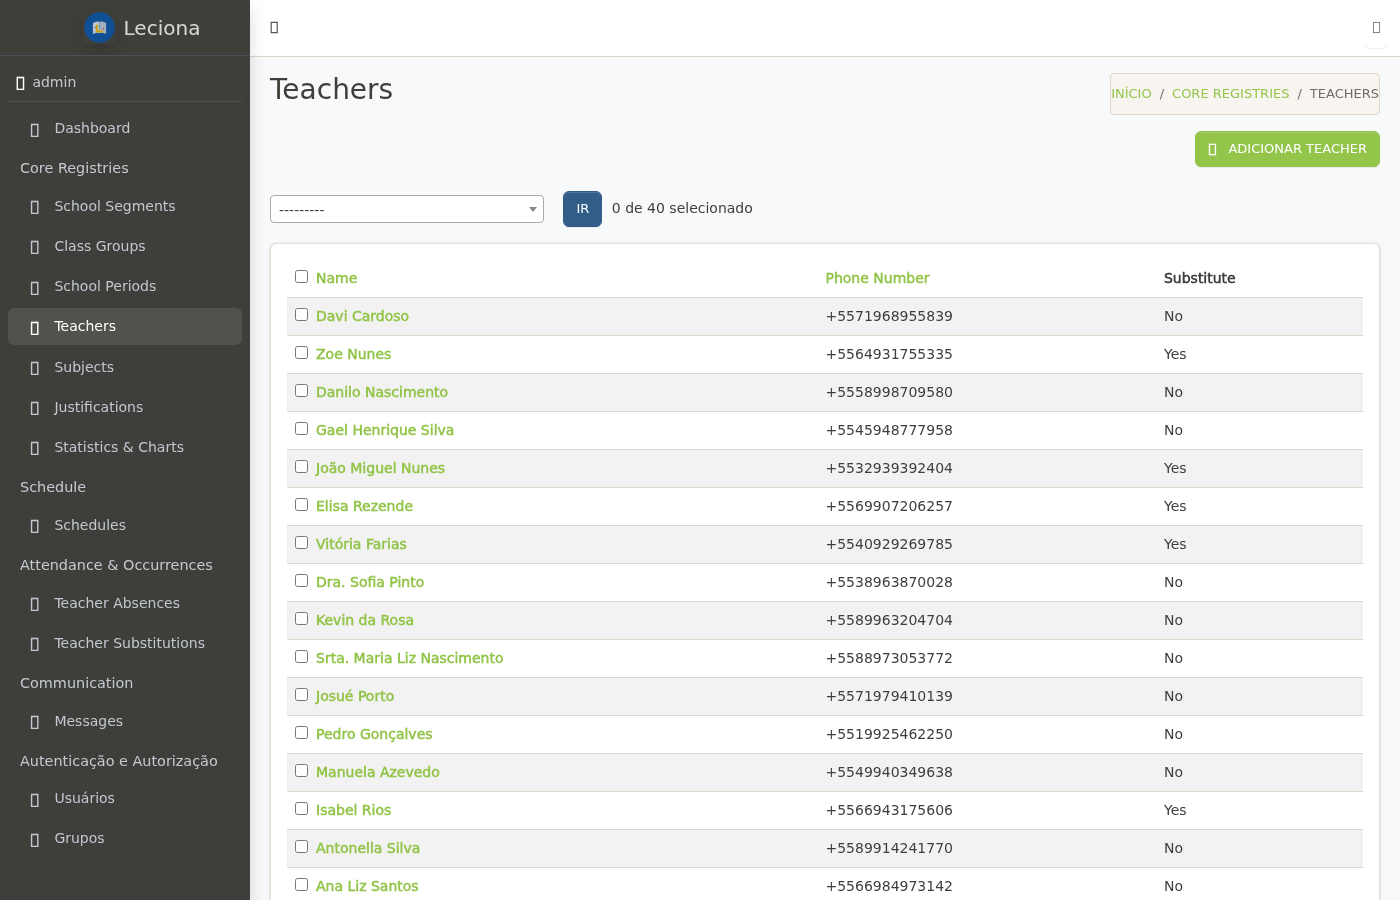
\includegraphics[width=0.9\textwidth]{images/teacher-list.png}
\caption{Lista de professores cadastrados no painel administrativo do Leciona}
\label{fig:teachers}
\end{figure}

\textbf{Gestão de horários com validação de conflitos.} O cadastro de horários pelo painel administrativo passa por validação em duas camadas. Na primeira camada (aplicação), o método \texttt{clean()} do modelo Schedule verifica que o horário de início é anterior ao horário de término e que o professor está habilitado a lecionar a disciplina indicada. Na segunda camada (banco de dados), as \texttt{UniqueConstraint} impedem a inserção de registros que gerariam choque de professor ou choque de turma. Quando uma tentativa de inserção viola alguma dessas restrições, o Django exibe uma mensagem de erro descritiva no formulário, sem que o registro inválido seja persistido.

\begin{figure}[H]
\centering
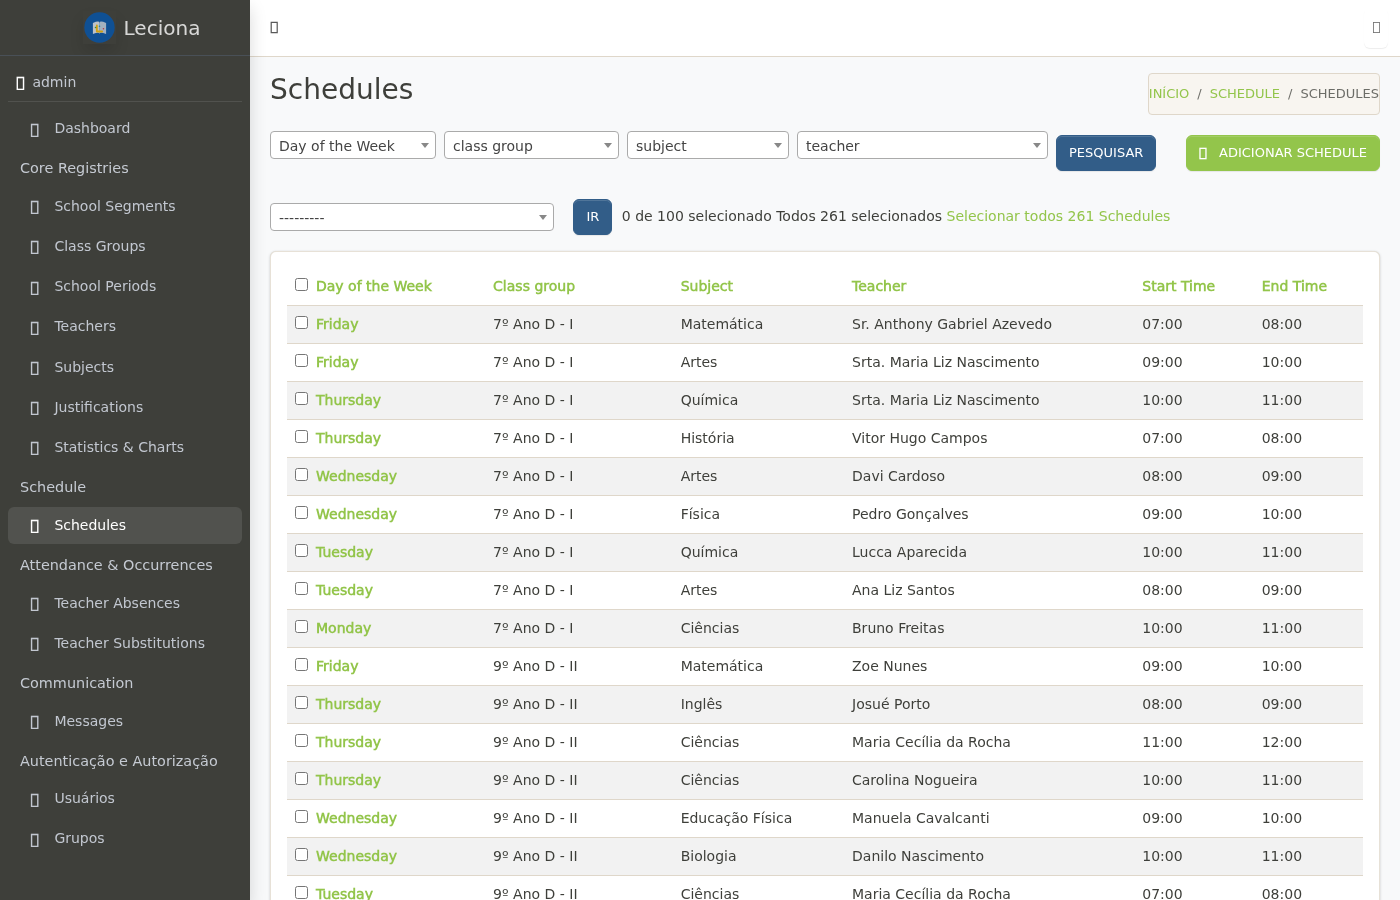
\includegraphics[width=0.9\textwidth]{images/schedule-management.png}
\caption{Lista de horários cadastrados com filtros por dia da semana, turma, disciplina e professor}
\label{fig:schedule}
\end{figure}

\textbf{Conteinerização com Docker.} O ambiente completo do Leciona pode ser iniciado com o comando \texttt{docker-compose up -d --build}. O Docker Compose orquestra dois serviços: \texttt{db} (imagem \texttt{postgres:15-alpine}, porta 5433, volume persistente) e \texttt{web} (imagem construída a partir do Dockerfile do projeto, porta 8080). Em desenvolvimento, o comando do serviço \texttt{web} é sobrescrito para utilizar o servidor de desenvolvimento do Django (\texttt{runserver}); em produção, o Dockerfile define o Gunicorn com três \textit{workers} como servidor padrão. O \textit{seed} de dados é executado dentro do contêiner com \texttt{docker-compose exec web python manage.py seed\_db}.

\textbf{Seed de dados realistas.} O comando \texttt{seed\_db} gera um conjunto de dados compatível com o cenário real da escola parceira: 40 professores (25\% marcados como substitutos) com nomes e telefones brasileiros gerados pelo Faker, 20 turmas vinculadas a 4 segmentos e 4 períodos, 11 disciplinas, 6 tipos de justificativa, horários de aula distribuídos de segunda a sexta em faixas de 07h às 12h (com tratamento automático de conflitos de \texttt{UniqueConstraint}), 50 ausências nos últimos 180 dias (70\% com substituição associada) e 20 comunicados. Esse conjunto permite testar todos os gráficos do dashboard com dados volumétricos e variados, além de validar o comportamento das restrições de integridade sob carga.

\textbf{Integração Contínua.} O pipeline de CI foi configurado via GitHub Actions no arquivo \texttt{.github/workflows/ci.yml}. O \textit{workflow} é acionado a cada \textit{push} e a cada abertura de \textit{pull request}, executando a suíte de testes do Django em um ambiente com PostgreSQL configurado como serviço. Essa automação garante que regressões sejam detectadas antes da integração ao ramo principal, reduzindo o risco de introdução de defeitos no código em produção.

\textbf{Acessibilidade.} A adoção do tema Jazzmin, construído sobre o AdminLTE 3 e o Bootstrap 4, confere ao painel administrativo uma interface responsiva com suporte a atributos ARIA, \textit{labels} associados a campos de formulário, contrastes de cor adequados e navegação por teclado. Embora uma auditoria formal de conformidade com as WCAG 2.1 ainda não tenha sido realizada, as escolhas tecnológicas adotadas fornecem uma base sólida para acessibilidade, que será avaliada com maior rigor nas próximas iterações.

\textbf{API RESTful.} Até o momento, o endpoint \texttt{/chartJSON/} constitui o primeiro ponto de acesso à API, servindo dados de ausências e substituições em formato JSON para consumo assíncrono pelo Chart.js. A expansão da API com endpoints dedicados para consulta de horários, ausências e substituições por interfaces externas está planejada para as próximas quinzenas, dando continuidade ao objetivo de transformar o sistema em uma plataforma orientada a serviços.

\textbf{Deploy em nuvem.} A conteinerização com Docker e Docker Compose, já funcional, representa a etapa preparatória para o deploy em nuvem. O ambiente está configurado de forma que a mesma imagem utilizada localmente possa ser implantada em qualquer provedor de nuvem (AWS, GCP, Railway, entre outros) sem alterações na configuração. A efetivação do deploy remoto está prevista para as próximas iterações do projeto.

Em síntese, os resultados parciais demonstram que o sistema Leciona evoluiu de um protótipo local para uma aplicação conteinerizada, com restrições de integridade, dashboard analítico, exportação de relatórios, pipeline de integração contínua e o primeiro endpoint de API JSON. A validação junto à escola parceira, prevista para a Quinzena 4, fornecerá o \textit{feedback} necessário para as últimas iterações do projeto dentro do semestre.


% ═══════════════════════════════════════════════════════════════════════════════
\section[Considerações parciais]{CONSIDERAÇÕES PARCIAIS}
% ═══════════════════════════════════════════════════════════════════════════════

O desenvolvimento do sistema Leciona no contexto do Projeto Integrador III encontra-se em estágio avançado de execução. Dos oito objetivos específicos definidos, seis já foram total ou parcialmente alcançados: a refatoração em módulos independentes (objetivo 1), a implementação de restrições de integridade no banco de dados (objetivo 2), o dashboard analítico com gráficos dinâmicos (objetivo 3), a conteinerização com Docker (objetivo 4), a exportação de relatórios em PDF (objetivo 7) e a configuração do pipeline de integração contínua (objetivo 6).

Dois objetivos estão em andamento e serão concluídos nas próximas quinzenas: a expansão da API RESTful com endpoints dedicados para consumo externo de dados (objetivo 5) e a validação da solução junto à comunidade escolar (objetivo 8), prevista para a Quinzena 4. Adicionalmente, a efetivação do deploy em um provedor de nuvem complementará a conteinerização já realizada, permitindo que a escola parceira acesse o sistema remotamente.

As principais contribuições técnicas obtidas até o momento incluem a arquitetura modular com separação clara de responsabilidades, a proteção em duas camadas contra inconsistências de dados (aplicação e banco), e a geração de indicadores visuais que subsidiam a tomada de decisão da equipe gestora. O \textit{feedback} da escola parceira, a ser coletado na próxima etapa, orientará os ajustes finais e a priorização das funcionalidades remanescentes.
